\documentclass[border=5pt]{standalone}
\usepackage{tikz}
\usepackage{amsmath}
\usetikzlibrary{positioning, arrows.meta, calc, fit, backgrounds}

% --- Color Scheme (Blue-Gray) ---
\definecolor{bgPrimary}{HTML}{DAE8FC}
\definecolor{bgSecondary}{HTML}{E8EEF7}
\definecolor{bgAccent}{HTML}{B3CDE3}
\definecolor{bgInput}{HTML}{F0F4F8}
\definecolor{borderPrimary}{HTML}{6C8EBF}
\definecolor{borderAccent}{HTML}{3A6EA5}
\definecolor{arrowColor}{HTML}{4A6A8A}
\definecolor{textMain}{HTML}{2C3E50}
\definecolor{textLight}{HTML}{7F8C8D}
\definecolor{bgHighlight}{HTML}{FFF3CD}

% --- Styles ---
\tikzset{
  module/.style={
    draw=borderPrimary, fill=bgPrimary, rounded corners=4pt,
    minimum width=2.8cm, minimum height=1.4cm,
    font=\sffamily\small, text=textMain, line width=0.6pt, align=center,
  },
  novelmodule/.style={
    draw=borderAccent, fill=bgAccent, rounded corners=4pt,
    minimum width=2.8cm, minimum height=1.4cm,
    font=\sffamily\small\bfseries, text=textMain, line width=1.0pt, align=center,
  },
  iobox/.style={
    draw=borderPrimary, fill=bgInput, rounded corners=3pt,
    minimum width=2.2cm, minimum height=1.0cm,
    font=\sffamily\small, text=textMain, line width=0.5pt, align=center,
  },
  lossbox/.style={
    draw=borderAccent, fill=bgHighlight, rounded corners=3pt,
    minimum width=1.8cm, minimum height=0.7cm,
    font=\sffamily\footnotesize, text=textMain, line width=0.5pt, align=center,
  },
  netblock/.style={
    draw=borderPrimary, fill=bgSecondary,
    minimum width=1.0cm, minimum height=0.5cm,
    font=\sffamily\tiny, text=textMain, rounded corners=2pt, line width=0.4pt, align=center,
  },
  stdarrow/.style={
    -{Stealth[length=5pt, width=4pt]}, line width=0.6pt, color=arrowColor,
  },
  lossarrow/.style={
    -{Stealth[length=4pt, width=3pt]}, line width=0.5pt, color=borderAccent, dashed,
  },
}

\begin{document}
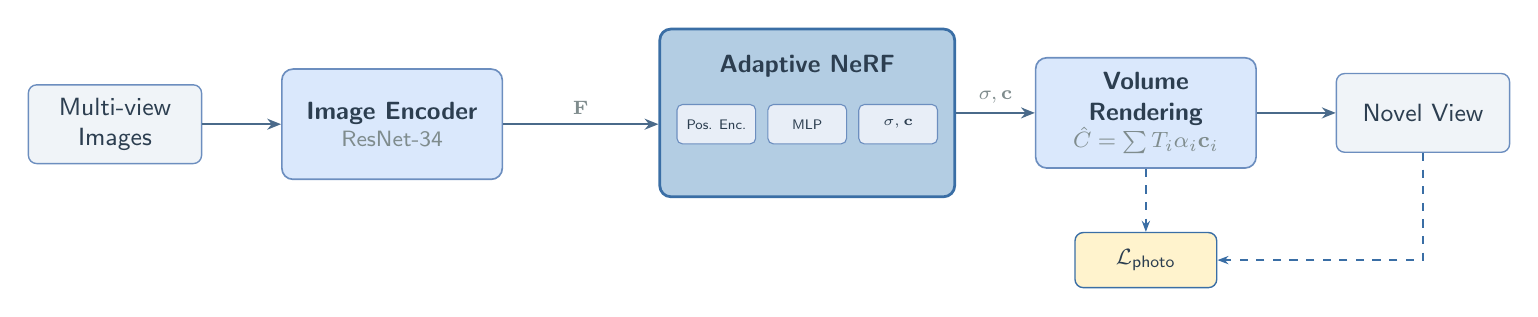
\begin{tikzpicture}

  % === Input ===
  \node[iobox] (input) {Multi-view\\Images};

  % === Feature Encoder ===
  \node[module, right=1.0cm of input] (encoder) {\textbf{Image Encoder}\\[-1pt]{\footnotesize\color{textLight}ResNet-34}};

  % === Novel: Adaptive NeRF — use fit to auto-size around sub-blocks ===
  % First place sub-blocks relative to encoder, then use fit to wrap them
  \node[netblock, right=2.2cm of encoder] (mlp1) {Pos. Enc.};
  \node[netblock, right=4pt of mlp1] (mlp2) {MLP};
  \node[netblock, right=4pt of mlp2] (mlp3) {$\sigma, \mathbf{c}$};

  % Title node above sub-blocks
  \node[font=\sffamily\small\bfseries, text=textMain, above=6pt of mlp2] (nerftitle) {Adaptive NeRF};

  % Invisible vertical anchor points at the same height as encoder, positioned at mlp2's x
  \coordinate (nerf_top) at (mlp2.center |- encoder.north);
  \coordinate (nerf_bot) at (mlp2.center |- encoder.south);

  % Fit node wrapping title, sub-blocks, and vertical anchors — drawn on background layer
  % so it doesn't cover the sub-blocks
  \begin{pgfonlayer}{background}
    \node[novelmodule, fit=(nerftitle)(mlp1)(mlp2)(mlp3)(nerf_top)(nerf_bot), inner sep=6pt] (nerf) {};
  \end{pgfonlayer}

  % === Volume Rendering ===
  \node[module, right=1.0cm of nerf] (render) {\textbf{Volume}\\{\textbf{Rendering}}\\[-1pt]{\footnotesize\color{textLight}$\hat{C}=\sum T_i\alpha_i\mathbf{c}_i$}};

  % === Output ===
  \node[iobox, right=1.0cm of render] (output) {Novel View};

  % === Loss ===
  \node[lossbox, below=0.8cm of render] (loss) {$\mathcal{L}_{\text{photo}}$};

  % === Arrows ===
  \draw[stdarrow] (input) -- (encoder);
  % Force horizontal: encoder.east → nerf.west at encoder's y-level (fit node center may be offset)
  \draw[stdarrow] (encoder.east) -- node[above, font=\sffamily\scriptsize, text=textLight] {$\mathbf{F}$} (nerf.west |- encoder.east);
  \draw[stdarrow] (nerf) -- node[above, font=\sffamily\scriptsize, text=textLight] {$\sigma, \mathbf{c}$} (render);
  \draw[stdarrow] (render) -- (output);

  % Loss arrows
  \draw[lossarrow] (render.south) -- (loss.north);
  \draw[lossarrow] (output.south) |- (loss.east);

\end{tikzpicture}
\end{document}
